% Cell-level Poisson DiD: spec + event-study results + HonestDiD
% (also hosts the METR-capability frame and the agentic re-anchor)

\begin{frame}{Empirical specification}
\begin{itemize}\setlength{\itemsep}{4pt}
  \item Cells: (occupation $j$ $\times$ age group $a$ $\times$ month $t$), private sector, 2021m1--2026m4
  \item One Poisson PPML regression per decade age group:
\end{itemize}
\[
\log E[\text{count}_{j,a,t}] = \alpha_{j} + \beta_{t} + \gamma_{q(j),\,k(t)}
\]
\begin{itemize}\setlength{\itemsep}{3pt}
  \item $\alpha_j$: occupation FE, absorbs permanent occupation size
  \item $\beta_t$: month FE, absorbs the aggregate age-cohort time path
  \item $\gamma_{q,k}$: log-point change for quintile $q$ at event time $k$, relative to \textbf{Q1} (least exposed) and $k = -1$ (October 2022)
  \item SE clustered at occupation
\end{itemize}

\vspace{0.2em}
\footnotesize
\textbf{Why Poisson?} Counts with some zeros; $\log(0+x)$ biased.\quad
Q3 (median) reference in backup.\quad\hyperlink{cell-es-q3-detail}{\beamerbutton{Q3 reference}}
\end{frame}

% ---------------------------------------------------------------
\begin{frame}{Cell-level event-study grid (Q1 reference)}
\hypertarget{after-cell-did}{}
\centering

\includegraphics[height=5.6cm,keepaspectratio]{figure_microdata_poisson_es_grid.pdf}

\vspace{0.2em}
\footnotesize
Q2--Q5 vs.\ Q1, by decade age group, private sector; reference October 2022 ($k=-1$). At 21--30, Q5 is noisy and ends near zero; 31--40 rises to about $+0.15$; 41--50 reaches about $-0.08$ by mid-2025 and ends near $-0.03$; 51--60 stays near zero.
\end{frame}

% ---------------------------------------------------------------
\begin{frame}{Difference-in-differences: Q5 vs.\ Q1, post-ChatGPT average}
\centering
\setlength{\tabcolsep}{8pt}
\begin{tabular}{lcccc}
\toprule
 & 21--30 & 31--40 & 41--50 & 51--60 \\
\midrule
Q5 $\times$ Post & 0.020 & 0.081*** & $-0.015$ & 0.010 \\
                 & (0.023) & (0.019) & (0.017) & (0.017) \\
\midrule
Occupations & 391 & 393 & 393 & 392 \\
\bottomrule
\end{tabular}

\vspace{0.8em}
\begin{itemize}\setlength{\itemsep}{4pt}
  \item Stacked triple difference, Q5 $\times$ Post $\times$ young (21--30 vs.\ 31--60): $-0.009$ (0.016), n.s.
  \item No larger post-ChatGPT decline for young workers in the most exposed quintile.
\end{itemize}

\vspace{0.2em}
\footnotesize
Poisson, occupation and month FE, SE clustered at occupation. *** $p<0.01$.
\end{frame}

% ---------------------------------------------------------------
\begin{frame}{Pre-trends are not parallel. How much does it matter?}
\small
\begin{itemize}\setlength{\itemsep}{2pt}
  \item Joint tests reject parallel pre-trends in every age group; the Q5 pre-period path moves 0.11 to 0.18 log points, as large as the post-2022 movements.
  \item HonestDiD (Rambachan \& Roth 2023): post-period average Q5 vs.\ Q1, ages 21--30.
\end{itemize}

\vspace{0.2em}
\centering
\footnotesize
\renewcommand{\arraystretch}{0.95}
\begin{tabular}{lc}
\toprule
Restriction & Robust 95\% CI \\
\midrule
Original ($\bar{M}=0$, parallel trends) & [-0.022, +0.065] \\
$\bar{M}=0.5$ & [-0.221, +0.301] \\
$\bar{M}=1.0$ & [-0.475, +0.555] \\
$\bar{M}=1.5$ & [-0.729, +0.796] \\
$\bar{M}=2.0$ & [-0.983, +1.064] \\
\midrule
Breakdown $\bar{M}$ & 0.00 \\
\bottomrule
\end{tabular}


\vspace{0.3em}
The conventional interval already includes zero, so there is no gradient to overturn (breakdown $\bar M = 0$). But the null is tight only under parallel trends: the robust intervals do not rule out large effects in either direction.
\end{frame}

% ---------------------------------------------------------------
\begin{frame}{AI capability is accelerating}
\centering
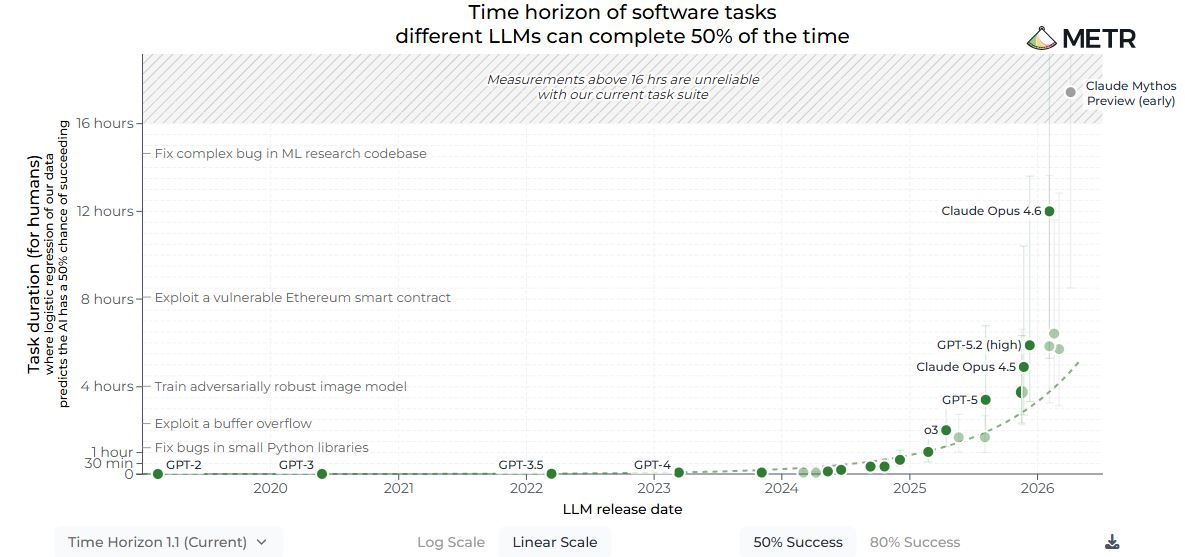
\includegraphics[height=5.5cm,keepaspectratio]{METR_time_horizon.JPG}

\vspace{0.4em}
\footnotesize
Length of software tasks an LLM completes at 50\,\% success has roughly doubled every $\sim$7 months since GPT-2. By 2026, the frontier handles multi-hour tasks. Source: Model Evaluation \& Threat Research (METR).
\end{frame}

% ---------------------------------------------------------------
\begin{frame}{Why agentic AI is a separate window}
\textbf{Mechanism.} Pre-agentic AI: AI helps with particular steps of a production chain, humans verify each step. Agentic AI: humans verify only the final output of a chain (Demirer, Horton, Immorlica \& Lucier 2026).

\vspace{0.6em}
\textbf{When did this happen?} Somewhat arbitrary, user cost falls gradually.
\begin{itemize}\setlength{\itemsep}{2pt}\footnotesize
  \item \textbf{Early 2024.} Devin demo (Mar 2024), Claude 3 Opus (Mar 2024), standardised function-calling APIs. Chaining technically possible but demo-grade.
  \item \textbf{May 2025.} OpenAI Codex (\href{https://openai.com/index/introducing-codex/}{16 May 2025}) and Anthropic Claude 4 / Claude Code (\href{https://www.anthropic.com/news/claude-4}{22 May 2025}) make multi-step coding agents production-grade.
\end{itemize}
\end{frame}

% ---------------------------------------------------------------
\begin{frame}{Re-anchor to agentic AI (April 2025)}
\centering

\includegraphics[height=5.6cm,keepaspectratio]{figure_microdata_es_decade_agentic.pdf}

\vspace{0.2em}
\footnotesize
Same Poisson DiD, re-anchored to April 2025 (last pre-agentic month). Pre-period 2023m1--2025m4, post 2025m5--2026m2. Cell-level, private sector. Q3 reference, estimated on data through February 2026.
\end{frame}
